\section{User Studies}
\label{sec:userstudies}


%%%%%%%%%%%%%%%%%%%%%%%%%%%%%%%%%%%%%%%%%%%%%%%%%%%%%%%%%%%%%%%%%%%%%%%%%%%%%%%%


We now expand our evaluations to a set of IRB-approved user studies. 
%
Here, we analyze the power savings and usability of {\myit} (and each of its features separately) under various scenarios. 
%
For this purpose, we use three types of applications: a static scene app,
a dynamic/interactive scene app, and one where users were given tasks that relate 
to the fidelity of the objects displayed in the scene. Videos of the apps are in \url{http://is.gd/logr\_mobisys}. 
%
Each experiment runs applications using five different configurations in
randomized order for each participant: 
%
(1) with {\myit}, 
(2) with {\myit} culling only, 
(3) with {\myit} frame rate control only, 
(4) with {\myit} mesh simplification only, and 
(5) without {\myit} (the native graphics rendering process). 
%
% The static application, in which we ask the users to observe static (floating)
% objects while rotating their heads, represents an application where {\myit} 
% can benefit the system performance the most. On the other hand, the dynamic 
% application, a simple game in which the users use the controller to pop sphere
% balls that fly towards the user from each side, represents a worst case
% scenario for {\myit} with high motion dynamics and large amounts of head motion.
% Finally, the object fidelity-based task application was designed to confirm that
% using {\myit} does not degrade the detailed fidelity of complex objects 
% while saving energy. 
%
Our user study involved 25 participants (avg.age: 24.6, 10 female) and the 
overall time to complete an experiment (per-user) was $\sim$30~mins with a \$10 
reward. At the end of each stage testing phase, users provided their subjective scores regarding the scene quality on a 5-point \emph{Likert scale} (very poor:1, very good:5).
%, and the energy usage is recorded using the {\mlo} energy profiler.
%
%\jp{'one stage' is per app? or per setting? or per app\&setting?}
%
%Additional values that we present related to the system's performance was 
%logged during the user studies as well. \jp{what other values?}


\begin{figure}[t]
    \centering
    \vspace{-2ex}
    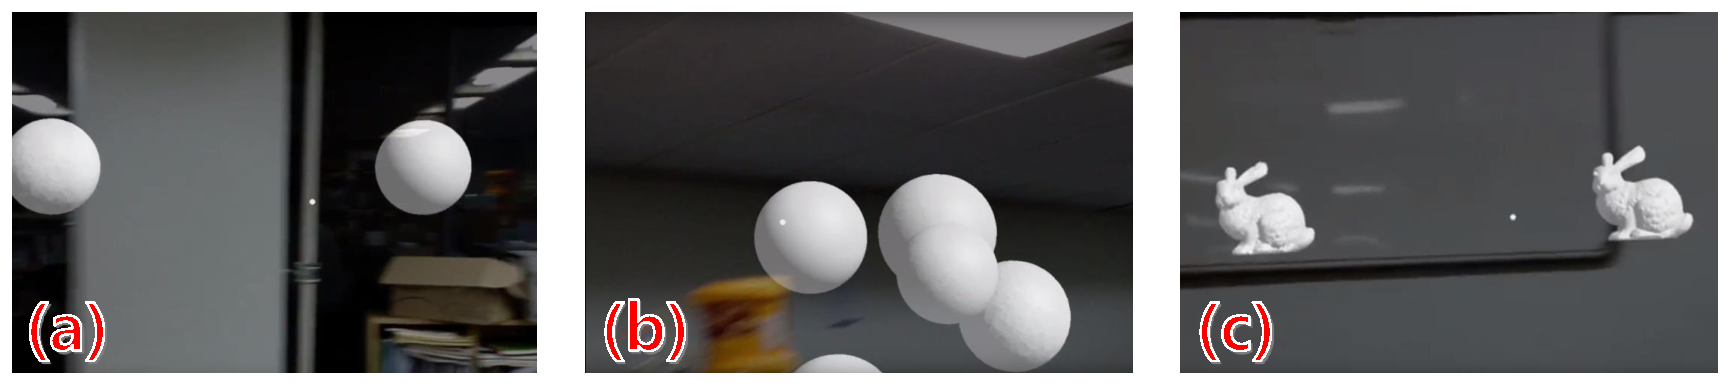
\includegraphics[width=1\linewidth]{scheme2_cropped}
    \vspace{-6ex}
    \caption{Screenshot from our three applications}
%            \jp{please insert some white space (gap) between images}}
    \label{fig:application}
\end{figure}


%%%%%%%%%%%%%%%%%%%%%%%%%%%%%%%%%%%%%%%%%%%%%%%%%%%%%%%%%%%%%%%%%%%%%%%%%%%%%%%%

\subsection{Static Scene App: Floating Spheres}

The purpose of the static scene application (the first app presented to all participants),
was to introduce and familiarize study participants to the mobile AR environment.
%
No specific tasks were given while the users slowly gazed through the 16 spheres
(69K triangles) that float (no dynamics) around the user (equally distributed 
over 360$^\circ$). Each of the five configurations was used for 30 seconds with
short breaks to answer user perception questions after each configuration.


\begin{figure}[t]
    \centering
    \vspace{-2ex}
    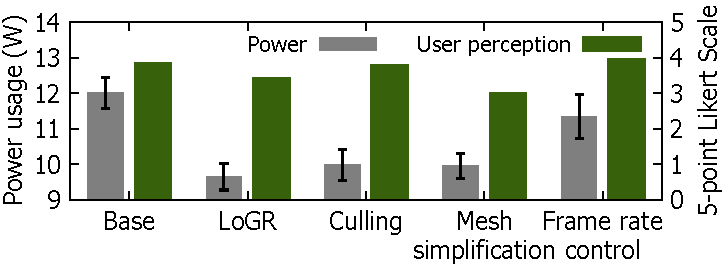
\includegraphics[width=0.8\linewidth]{static_energy_cropped}
    \vspace{-3ex}
    \caption{Mean power usage and user satisfaction scores in 5-point 
            \emph{Likert scale} for static scene app.}
    \label{fig:user-static}
\end{figure}

\fig\ref{fig:user-static} presents the mean power usage and user perception 
results for each test case. 
%
It shows that {\myit} can reduce power consumption by $\sim$22\% ($\sim$2.6~W) 
compared to the baseline graphics rendering process, and the mesh simplification
and culling sub-components contribute heavily to the power savings. 
%
This is because, for the static scene app, the spheres that are not in
the participants' core FOV can be culled or simplified, which leads to 
a significant reduction in GPU and memory usage. From the system lifetime perspective, the results for the baseline translates to 3.0 hours of operation time, and {\myit} adds 0.9 additional hours of operation. 
%

Finally, we can see that the user perceived quality level reports for {\myit} scored 3.54 compared to 3.80 for the baseline, but, this difference was not statistically significant (2-tailed t-test, p<0.05).

%While not significantly different, we explain this difference as the following. In the static scene app, there was no specific task given to the participants, and therefore the they focused closely to the object quality and some were distracted when neighboring spheres were presented in simplified form. This issue is even more prominent when we see the scores for the ``mesh simplification only'' case as well.

%are similar between 3.5-3.9 across all testing configurations.


%%%%%%%%%%%%%%%%%%%%%%%%%%%%%%%%%%%%%%%%%%%%%%%%%%%%%%%%%%%%%%%%%%%%%%%%%%%%%%%%

\subsection{Dynamic Scene App: Sphere Shooting}

The second application is a simple shooting game in which moving spheres fly into the 
scene, and participants are asked to use the controller and
their gaze to ``shoot'' and eliminate the spheres.
%
We design the application so that the spheres to appear in various patterns, in 
high-speeds, low-speeds, from the right and left, etc. %\jp{what kind of bias is this?}
%
Compared to static scenes, this application introduces both dynamics 
and interactive complexity.
%
Again, we test with the five configurations mentioned above and measure the power usage, 
user perception level and the hit/miss rate to quantify task accomplishment levels. 

%The second is a dynamic application like shooting games. This application allows the user to remove the balls coming from left and right sides through the controller. To understand hole energy consumption of that five stage's character, we designed five section in one stage such as default mode, high speed ball mode, low speed ball mode, a lot of balls on the left mode, a lot of balls on the right mode. We asked participants for this study to play the game in 30 seconds.


\begin{figure}[t]
    \centering
    \vspace{-2ex}
    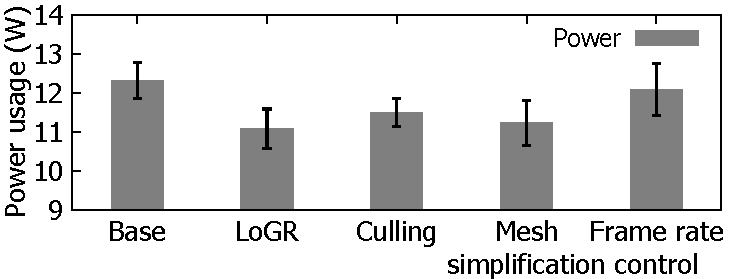
\includegraphics[width=0.75\linewidth]{dynamic_energy_cropped}
    \vspace{-3ex}
    \caption{Mean power usage for dynamic/interactive scene application.}
    \label{fig:user-dynamic-energy}
\end{figure}

%\jp{we are using 'W'... which is a unit of power, not energy.
%we may say 'energy consumption(rate)', but be careful not to say 'energy'}

\fig\ref{fig:user-dynamic-energy} plots the mean power consumption of this 
experiment with standard deviations.
%
Results show that the frame rate component shows only minimal power reduction of 2\%, 
noticeably less than 7\% for the static scene app results in \fig\ref{fig:user-static}. 
%
This is a result of having dynamic scenes, as {\myit} tries to adapt to such 
scenes with high frame rates to preserve application quality.
%
As in the static scene application case, the culling and frame rate control 
plays an important role; as the users focus on the spheres that
they shoot, other spheres can be simplified or culled. Overall, {\myit} 
saves $\sim$11\% power compared to the baseline consumption on average. 


\begin{figure}[t]
    \centering
    \vspace{-2ex}
    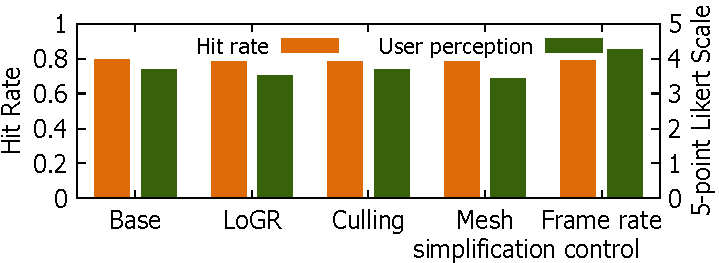
\includegraphics[width=0.85\linewidth]{dynamic_like_hit_cropped}
    \vspace{-2ex}
    \caption{Hit rate and user perception in 5-point Likert scale for dynamic/interactive scene app.}
    \label{fig:user-dynamic-usability}
\end{figure}


In \fig\ref{fig:user-dynamic-usability} we present the mean hit/miss rates 
with the user perception levels. Despite changing the configurations,
there is no noticeable change in the task accomplishment performance 
(i.e., hit rate) and the user perception is kept high across the different test cases.
%
%Compared to the static scene app, in this case, the users were focusing on a more specific task; thus, the small quality degradation did not disturb the quality of executing the target task.

%as well. \jk{potentially add wongyo's comment here}



%%%%%%%%%%%%%%%%%%%%%%%%%%%%%%%%%%%%%%%%%%%%%%%%%%%%%%%%%%%%%%%%%%%%%%%%%%%%%%%%


\subsection{Fidelity-centric App: Bunny Search}


\begin{figure}[t]
    \centering
    %\vspace{-2ex}
    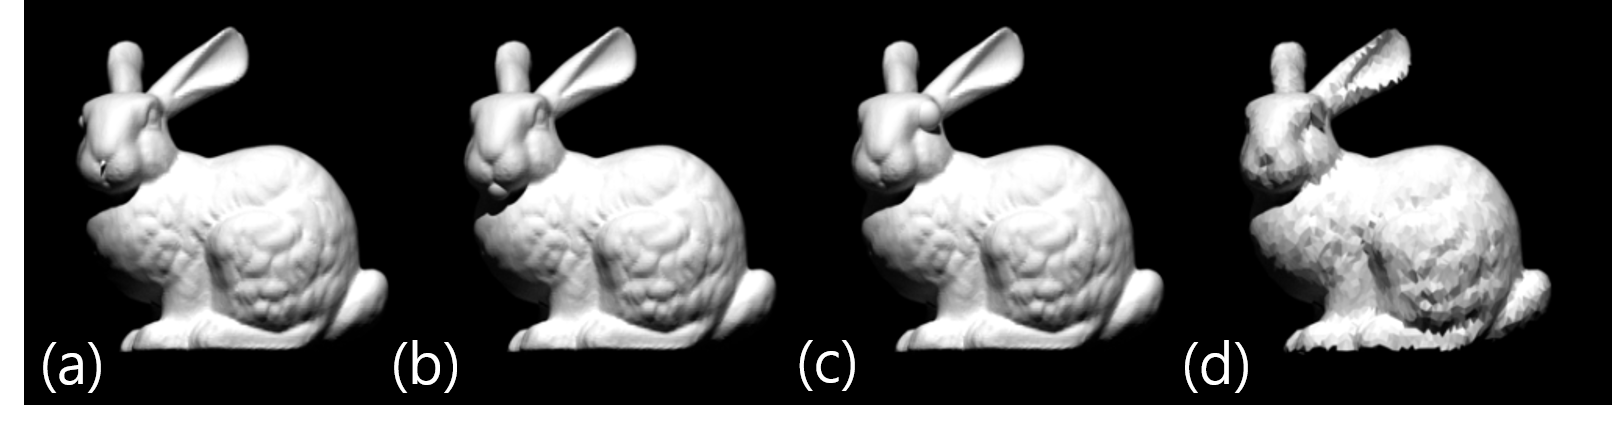
\includegraphics[width=0.9\linewidth]{abnormal_bunnies}
    \vspace{-4ex}
    \caption{Abnormal bunnies designed for our user studies (a)-(c).
            Example of the reduced triangle bunny used for
            the na\"{\i}ve power reduction tests (d).}
    \label{fig:user-bunny}
\end{figure}


The third application used in our user study was designed to conceptualize a group
of real world AR applications in which the fidelity of the displayed object quality 
impacts task accomplishment performance.
%
Specifically, as \fig\ref{fig:user-bunny} shows, we made small, but noticeable,
changes to the original Stanford Bunny by adding small spheres to the eyes or mouth.
%
In the scene, we uniformly distribute 16 bunnies (mixture of normal and abnormal) in 
the 360$^\circ$ space.
%
Study participants would need to look close to the details of each bunny to identify the abnormalities. 
%
We then ask study participants to locate \textit{two} abnormal bunnies with the same 
abnormality. These bunnies are located at least 120$^\circ$ away
from each other to avoid cases where they are adjacent. 
%
We ask for two that are apart (instead of one) to avoid the case where 
an abnormal bunny is located closely at the view point at the beginning of the experiment; 
thus, easy to find with minimal effort.
%
With such scenario, we run three experiments which include 
(1) {\myit}, 
(2) baseline rendering, and 
(3)  na\"{\i}ve power reduction.
%
In the na\"{\i}ve power reduction case, we use the baseline rendering, 
but display bunnies with fewer triangles so that the power usage of the {\mlo}
matches {\myit} (c.f., \fig\ref{fig:user-bunny}).
%
At the beginning of each test, we let the participant know what type of
abnormality they are to find (among the three types), and record the power usage 
and search times until the task successfully completes. Note that prior to performing the three test cases, we allowed the participants to perform one practice run with the baseline rendering mode, so that they well-understood the target task. 


\begin{figure}[t]
    \centering
    \vspace{-2ex}
    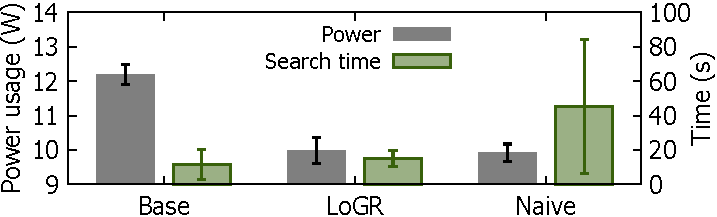
\includegraphics[width=0.8\linewidth]{fidelity_energy_cropped}
    \vspace{-3ex}
    \caption{Mean power consumption and time consumed to accomplish 
            abnormal bunny search task.}
    \label{fig:user-fidelity}
\end{figure}


We present the mean power consumption and the task accomplishment
times in \fig\ref{fig:user-fidelity}.
%
When using {\myit}, we save approximately 20\% in energy compared to the 
baseline. At the same time, the time taken to accomplish the task
was not noticeably affected (11 seconds for baseline 13 seconds for {\myit}).
%
On the other hand, when comparing {\myit} against the 
na\"{\i}ve power reduction case, the power consumption of the two are
similar, but the task completion time differ by more than three-fold.
%
Given that the na\"{\i}ve power reduction case simplifies all displayed 
objects uniformly (see \fig\ref{fig:user-bunny}(d)), identifying the abnormal bunny 
becomes bigger challenge than before, whereas {\myit} reduces power usage while preserving the user perceived scene quality by exploiting the head and gaze orientation data from the mobile headset. 


%The last is a finding bunny that is looking for two bunnies with the features we asked in 16 bunnies. we batched two bunnies with the features because of reducing effect of bunnies space in starting time. For example, when start the game bunnies is located in front of users, the time of game is too short. In this experiments, we wanted to understand different of energy consumption of full {\myit} and no {\myit} and the time it takes to apply bunnies of lower quality to the same application to achieve energy efficiency of {\myit}. 

%\jk{Fig : energy + normalized search time}

%\jk{Fig : show bunny quality using pictures}


